\section{Chapter 6 - Problem (2)}

	A roller-coaster car has a mass of $1300 \ kg$ when fully loaded with passengers. As the car passes over the top of a circular hill of radius $19 \ m$, its speed is not changing.

	\subsection{Question (a)}

		At the top of the hill, what is the normal force on the car from the track if the car's speed is $v = 7.9 \ m/s$?

		\textbf{R:} \newline

		\begin{figure}[H]
			\begin{center}
				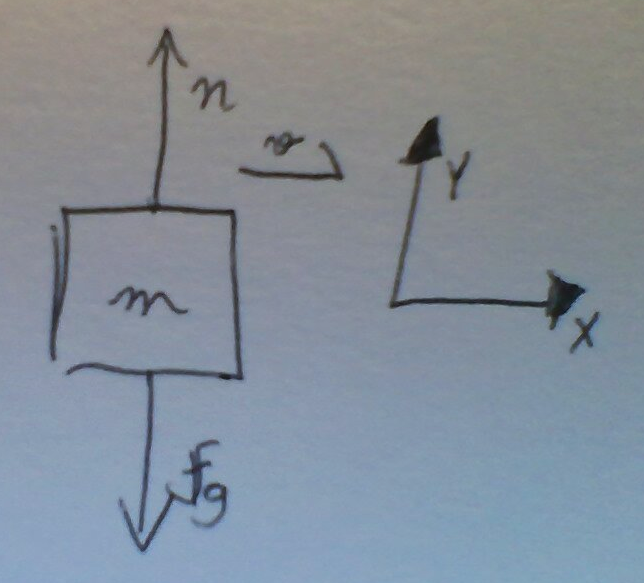
\includegraphics[scale=0.3]{hw6_problem2_fbd}
				\caption{Free-Body Diagram (Problem 2)}
				\label{fig:hw6_problem2_fbd}
			\end{center}
		\end{figure}

		Newton's $2^{nd}$ Law:
		\begin{align}
			\sum F_{y} = \ &ma_{y}& \notag \\
			n - mg = \ &ma_{c}& \notag \\
			n = \ &mg + ma_{c}& \notag \\
			= \ &m\left(g + \frac{v^{2}}{r} \right)& \notag \\
			= \ &(1300 \ kg)\left[\left(9.80 \ m/s^{2}\right) + \frac{(7.9 \ m/s)^{2}}{19 \ m} \right]& \notag \\
			= \ &(1300 \ kg)\left[\left(9.80 \ m/s^{2}\right) + \frac{62.41 \ m^{2}/s^{2}}{19 \ m} \right]& \notag \\
			= \ &(1300 \ kg)\left[\left(9.80 \ m/s^{2}\right) + (3.285 \ m/s^{2}) \right]& \notag \\
			= \ &(1300 \ kg)\left(13.085 \ m/s^{2} \right)& \notag \\
			= \ &17 \ 010.5 \ N&
		\end{align}

	\subsection{Question (b)}

		What is the normal force if $v = 17 m/s$?

		\textbf{R:} \newline

		\begin{align}
			n = \ &m\left(g + \frac{v^{2}}{r} \right)& \notag \\
			= \ &(1300 \ kg)\left[\left(9.80 \ m/s^{2}\right) + \frac{(17 \ m/s)^{2}}{19 \ m} \right]& \notag \\
			= \ &(1300 \ kg)\left[\left(9.80 \ m/s^{2}\right) + \frac{289 \ m^{2}/s^{2}}{19 \ m} \right]& \notag \\
			= \ &(1300 \ kg)\left[\left(9.80 \ m/s^{2}\right) + (15.211 \ m/s^{2}) \right]& \notag \\
			= \ &(1300 \ kg)\left(25.011 \ m/s^{2} \right)& \notag \\
			= \ &32 \ 514.3 \ N&
		\end{align}
